%\documentclass[11pt, twoside]{article}
\documentclass[11pt]{article}

\usepackage{amsmath} 
\usepackage{times}
\usepackage{amsmath,amsthm,amssymb}
\usepackage{enumerate}
\usepackage{fancyhdr}
\usepackage{moreverb}
\usepackage{graphicx}
\usepackage{verbatim}
\usepackage{amssymb}
\usepackage{url}
\usepackage{multirow} 
\usepackage[boxed, section]{algorithm}
\usepackage{algorithmic}
\usepackage{cite}
\usepackage{multirow} 
\usepackage{rotating}
\usepackage{geometry}
\usepackage{fix-cm}
\usepackage{natbib}

\usepackage{caption}
\usepackage{subcaption}
\usepackage{color}
\usepackage[T1]{fontenc}
\usepackage[utf8]{inputenc}
\usepackage{authblk}

\newcommand{\myN}{\hbox{N\hspace*{-.9em}I\hspace*{.4em}}}
\newcommand{\myZ}{\hbox{Z}^+}
\newcommand{\myR}{\hbox{R}}
\renewcommand{\P}{\mathbb{P}}
\newcommand{\E}{\mathbb{E}}
\newtheorem{defi}{Definition}
\newtheorem{theorem}{Theorem}[section]
\newtheorem{lemma}[theorem]{Observation}
\newtheorem{observation}[theorem]{Observation}
\newtheorem{proposition}[theorem]{Proposition}
\newtheorem{claim}[theorem]{Claim}
\DeclareMathOperator*{\argmax}{arg\,max}

\theoremstyle{definition}
\newtheorem{example}[theorem]{Example}
\theoremstyle{definition}
\newtheorem{definition}[theorem]{Definition}

\renewcommand{\abstractname}{}
\def\pb{\overline{p}}
\def\pt{\tilde{p}}
\def\one{{\bf 1}}
\def\F{{\cal F}}
\def\G{{\cal G}}
\def\P{{\mathbb P}}
\def\E{{\mathbb E}}
\def\Var{{\rm Var}\,}
\def\Cov{{\rm Cov}\,}
\def\ee{\varepsilon}
\def\|{\, | \,}
\def\probit{p_{\rm probit}}
\def\plog{p_{\rm log}}

%%%%%% Begin document with header and title %%%%%%%%%

\title{Combining Probability Forecasts and Understanding Probability Extremizing through Information Diversity}
\author[1]{Ville A. Satop\"a\"a\thanks{Corresponding author. tel.: +1 215 760 7263; fax: +1 215 898 1280; email: satopaa@wharton.upenn.edu}}
%\author[2]{Robin Pemantle\thanks{pemantle@math.upenn.edu}}
%\thanks{Research supported by NSF award \# DMS-1209117}
%\author[3]{Lyle H. Ungar\thanks{ungar@cis.upenn.edu}}
\author[2]{Robin Pemantle\thanks{Research supported in part by NSF grant
   \# DMS-1209117}}
\author[3]{Lyle H. Ungar}
\affil[1]{Department of Statistics,
The Wharton School of the University of Pennsylvania\\
400 Jon M. Huntsman Hall\\
3730 Walnut Street\\
Philadelphia, PA 19104-6340}
\affil[2]{Department of Mathematics\\
University of Pennsylvania\\
David Rittenhouse Laboratories\\ 
209 S. 33rd Street\\
Philadelphia, PA 19104-6395 }
\affil[3]{Department of Computer and Information Science\\
University of Pennsylvania\\
504 Levine, 200 S. 33rd Street\\
Philadelphia, PA 19104-6309}
\date{\vspace{-10ex}}


\begin{document}
\maketitle
\pagestyle{myheadings}
\markboth{Understanding Probability Extremizing}{Satop\"a\"a et al.}
\begin{abstract}
\noindent
\textbf{Summary.} Randomness in scientific estimation is generally 
assumed to arise from unmeasured or uncontrolled factors. However, 
when combining subjective probability estimates, heterogeneity
stemming from people's cognitive or information diversity is often
more important than measurement noise.  This paper presents a novel
framework that models the heterogeneity arising from forecasters that use 
partially overlapping information sources, and applies that model to 
the task of aggregating the probabilities given by a group of forecasters 
who forecast whether an event will occur or not. Our model describes 
the distribution of information across forecasters in terms of easily
interpretable parameters and shows how the optimal amount
of \textit{extremizing} of the average probability forecast (shifting
it closer to its nearest extreme) varies as a function of the forecasters'
information overlap.  Our model thus gives a more principled
understanding of the historically {\it ad hoc} practice of extremizing
average forecasts.\\
\\
\textit{Keywords:} forecaster Beliefs; Information Aggregation; Model Averaging; Probability Forecasting; Stochastic Process; Wisdom of Crowds
\end{abstract}


\section{Introduction and Overview}

\subsection{The Forecast Aggregation Problem}

Event forecasting is the science of giving probability forecasts
for future events.  The classical example is 
meteorological~\citep{sanders1963subjective},
predicting for example whether rain will occur in a given time period.
The practice is now common in many other fields, including
medical diagnosis~\citep{wilson1998prediction,pepe2003statistical} and
political and socio-economic event forecasting~\citep{tetlock2005forecaster};
for example, one might forecast the winner of the next Congolese election, 
whether war will break out in Egypt this year, and so forth.  

Such forecasting tasks typically involve several probability forecasts arising from diverse sources (e.g., statistical models, human forecasters, etc.). The decision maker then takes action based on this information. A typical first step, known as \textit{forecast aggregation}, is to combine the probabilities  into a single forecast with optimal properties. Bringing together the
strengths of different forecasters in this manner has been shown to improve predictive
performance under various contexts.~\citep{clemen1989combining, armstrong2001combining}.

There are two approaches to forecast aggregation: empirical
and theoretical.  The empirical approach is akin to machine
learning.  Given several forecast streams, the decision maker experiments
with different aggregation procedures, evaluates the results
of these on training data, and finally selects parameters values that optimize 
the results.  The theoretical approach, on the other hand, first produces a probability
model and then computes the optimal aggregation procedure under the 
assumptions of the model.  This may involve estimating parameters 
of the model from the data.  

Both approaches are important.  Procedures based on theory that
do not perform well in practice are ultimately of limited use.
On the other hand, an empirical approach without theoretical
underpinnings lack both credibility (why should we believe it?)
and guidance (in which direction can we look for improvement?).
As we will discuss below, the history of forecast aggregation
to date is largely empirical\footnote{Not only the approaches in
Section~\ref{ss:empirical} but also the approaches described in
Section~\ref{ss:measurement}, to which we have provided theoretical 
underpinnings, have been pursued in a manner that is largely empirical.}.  
The goal of this paper is to
produce a plausible theoretical framework for forecast aggregation.
This framework allows us to interpret existing aggregation 
procedures and illuminate aspects that can be improved.
Secondly, at a general level, we use this framework to shed light on 
the practice of {\em probability extremizing} (shifting an average aggregate closer to its nearest extreme). Thirdly, we apply
this framework to a specific toy model, where the optimal 
aggregator may be computed and reflects qualitative properties 

\subsection{Bias, Noise and Forecast Assessment}

A forecast is an estimator of an indicator function.  As is
the case with any estimator, its deviation from the truth
can be broken into two pieces: bias and noise.  A forecast
stream is said to be {\em calibrated}
if, in the long run, events associated with a forecast $p$ have an empirical frequency of occurrence of $p$ (see, e.g., \citealt{degroot1983comparison}). 
In the lingo of estimation, this is equivalent to being conditionally 
unbiased.  A forecast stream that is not calibrated
can, in principle, be corrected by translating the forecast $p$ into the forecast $\pt$
where $\pt$ is the (historical) proportion of times the 
event occurs when $p$ is forecast.  One can then assume without
loss of generality that the forecast stream is true, replacing
$p$ if necessary by the historically corrected $\pt$.

This assumption is, of course, valid only in principle: 
it relies on a relatively lengthy history and an assumption
of stationarity of the properties of the forecast.  Nevertheless,
on the theoretical level, it is important to separate the problems 
of bias and noise because they are solved by different mechanisms.
In this paper we consider the aggregation problem for calibrated forecast
streams, thus isolating the task to one of noise reduction.  

Before delving into the problem of forecast aggregation, it is useful to briefly discuss the problem of assessing and improving a single
forecast stream.  The most common methodology is to use a loss
function.  Letting $\one_A$ denote the indicator function of the
event $A$ being forecast, the loss function is a penalty 
$L(p , \one_A)$ where $p$ is the forecasted probability.
A loss function is said to be {\em revealing} or {\em proper}
if the Bayesian optimal strategy is to tell the truth.  In other words, 
if the subjective probability estimate is $p$, then $t = p$ should
minimize the expected loss $p L(t,1) + (1-p) L(t,0)$.  This expected loss is a one dimensional
assessment of an estimator. Many
choices, however, are possible, and an estimator that outperforms 
another under one loss function will not necessarily do so
under a different loss function.  For example, minimizing the quadratic loss function
$(p - \one_A)^2$, also known as the {\em Brier score}, gives the estimator with the least variance. On the other hand, minimizing the entropy loss $\log (1 / |p - \one_{A^c}|)$ reveals the estimator that best avoids forecasting an incorrect event with near 
certainty; see~\citet[Section~2]{HwPe1997} for a discussion of
proper loss functions.

The point of this brief review is two-fold.  First, when a group of
sophisticated forecasters operates under a revealing loss function,
the assumption of calibrated forecast streams is, to some degree, 
self-fulfilling.  Forecasters can improve their long run 
performance by calibrating their forecasts. Forecasters with 
competitive motivation, sophistication and historical data
will probably do so.  Secondly, the assessment of the aggregated forecast
is not uni-dimensional any more than is the assessment of an
individual forecast.  In order to compare different aggregation 
procedures, a scoring rule must be chosen.  In practice, the
Brier score is the most common choice, perhaps because of its simplicity
or because of the paramount status of variance in the statistical
literature.  In this paper we will concentrate on minimizing the
variance of aggregators, though much of the discussion will hold under
general proper loss functions.

\subsection{The Partial Information Model}

Any probability model for forecast aggregation must begin with a 
probability space $(\Omega, \F , \P)$ and a measurable event
$A \in \F$ to be forecasted.  In any Bayesian setup, with a proper 
loss function, it is more or less tautological that a forecaster
reports $p = \E (\one_A \| \G)$ where $\G \subseteq \F$ is the
information used by the forecaster.  Our most general model for
forecast aggregation is little more than this.  Suppose there are
$N$ forecasters, numbered $1, \ldots, N$.  We posit the existence
of sub-$\sigma$-fields $\F_i \subseteq \F$ such that Forecaster~$i$
forecasts $p_i = \E (\one_A \| \F_i)$.  Anything further must come from
assumptions on the structure of the collection $\{ \F_i \}_{i=1}^N$.
%%%In Section~?? we explore in detail a particular such structure.

This setup is quite flexible.  Suppose, for example, that there are
many events $A_1, A_2 , \ldots,$ to be forecasted.  For each event 
$A_j$, the model assumes only that Forecaster~$i$ uses some 
$\sigma$-field $\F_{ij}$.  Further aspects of the problem are
reflected by the structure of the collection $\{ \F_{ij} \}$.
For example, if the events are sequenced in time, then probably
$\{ \F_{ij} : j = 1 , 2, 3, \ldots \}$ will be an increasing 
sequence.  If the forecasts are public, it may make sense to 
asume that $\F_{ij}$ contains all forecasts up to time $j-1$.
If the forecasts of each individual $A_j$ are sequenced rather 
than synchronous, it may make sense for $\F_{ij}$ to include
some forecasts at time $j$ as well.  

If a forecaster uses a simple rule, the $\sigma$-field $\F_i$ may 
not be the full $\sigma$-field of information available to 
Forecaster~$i$ but rather a smaller $\sigma$-field corresponding
to the information actually used by the rule.  For example, 
when forecasting of the event of re-electing the president,
a forecaster obeying the dictum ``it's the economy, stupid!''
might be assigned a $\sigma$-field containing only economic indicators.
A forecasting automaton might use a similarly restricted subset
of the information fed to it.

In this model, we distinguish two benchmarks for efficiency in
aggregation.  The first is the {\em oracular} aggregator, which
forecasts $p' := \E (\one_A \| \F')$ where $\F'$ is the $\sigma$-field
generated by the union of the $\sigma$-fields $\{ \F_i : 1 \leq i 
\leq N \}$.  Obviously, it is not possible do better when forecasting the
probability of the event $A$ than to use all the information available 
to the forecasters; note that if a forecaster chooses to throw away 
some of the available information then, for purposes of aggregation,
the information may as well not exist.  The oracular aggregator
is a reasonable model for an upper bound on estimation efficiency;
information not in $\F'$ represents randomness inherent in the outcome.

In practice, the aggregator cannot necessary do as well as this.  
Information comes to the aggregator only via the forecasts.  Hence the 
aggregator cannot improve upon the estimate $p'' := \E (\one_A \| \F'')$
where $\F''$ is the $\sigma$-field generated by the forecasts
$\{ p_1 , \ldots , p_N \}$.  We call this the {\em revealed} aggregator 
because it uses exactly the information revealed by the forecasters
through their forecasts.  The {\em general partial information model} 
is precisely the model described in the foregoing paragaphs.  
Specific partial information models involve assumptions on
the structure of $\{ \F_i \}$.  In each case, the relevant estimator 
is the revealed aggregator. 

\subsection{Organization of the Paper}

In the next section we review some prior work on aggregation and 
indicate the relation to the partial information framework.
Section~\ref{sec:model} discusses some lliuminating toy examples 
and motivates our subsequent choices of specific partial information 
models.  Section~\ref{extremizing} compares the oracular
aggregator $p'$ with the average probit $\probit$, thereby
explaining the empirical practice of {\em probability extremizing}.
Section~\ref{aggregation} analyzes the revealed aggregator for a
particular specific toy partial information model.  We conclude
with a discussion section.


\section{Some Prior Work on Aggregation}
\label{sec:prior}

Prior work on aggregation has focused on non-quantitative
frameworks used to explain heterogeneity of subjective forecasts.  
We discuss two of these here.

\subsection{The Interpreted Signal Framework}
\label{ss:inerpreted}

\citet{hong2009interpreted} adopt the {\em interpreted 
signal framework} in which forecaster opinions are based on a personal
interpretation of (a subset of) the factors or cues that influence
the future event to be predicted.  Differences among forecaster
predictions are ascribed to differing interpretation procedures.
For example, if two forecasters follow the same political campaign
speech, one may focus on the content of the speech while the other 
may concentrate largely on audience interaction.  Even though the
two candidates both receive the same information, they interpret
it differently, arriving at different forecasts for the probability
that this candidate wins the election.  

Therefore, under the interpreted signal framework, forecast heterogeneity 
stems from cognitive diversity.  This is a realistic framework that
has been analyzed and extended to many other settings.  For example,
~\citet{parunak2013characterizing} demonstrate that 
forecast aggregation in this model is not constrained to the convex 
hull of the forecasts;~\citet{broomell2009forecasters}
analyze inter-forecaster correlation
under the assumption that the cues can be mapped to the forecasters'
forecasts via different linear regression functions.

The interpreted signal framework, when formalized, more or less implies 
the partial information model.  Unfortunately, previous work on
interpreted forecasts has produced only abstract concepts and 
has not been taken to the level of a precise formal model with 
quantitative predictions.  

\subsection{The Measurement Error Framework}
\label{ss:measurement}

Given the lack of a quantitative model for the interpreted signal framework, in practice it is often easier and more common to explain subjective
forecasts with the classical {\em measurement error framework}.  This framework assumes a ``true'' probability (interpreted
as the probability forecast made by an ideal forecaster) for the future 
event.  The forecasters are able to measure this probaiblity but with
some mean-zero idiosyncratic error.  Each forecast is then modeled
as a draw from a common probability distribution that is typically 
centered at the true probability.  
%
In other words, the underlying probability model is just the classical statistical
model for measurement with IID mean zero error.  Consequently, the average probability, $\pb = \frac{1}{N}\sum_{i=1}^N p_i$,
is an aggregator which will be unbiased and have the least variance.

Variants on this model alter the quantity that is supposedly 
measured without bias.  If instead of $p$, for example,
the log odds $\log (p/(1-p))$ has been measured without bias, 
the the average log odds will be an unbiased estimator for
the true log odds.  Transforming the average log odds back into
an estimate for $p$ yields the {\em logarithmic opinion pool}
$$\plog := \frac{\exp \left [ \frac{1}{N} \sum_{i=1}^N
   \log (p_i / (1-p_i)) \right ]}
{1 + \exp \left [ \frac{1}{N} \sum_{i=1}^N
   \log (p_i / (1-p_i)) \right ]} \, .$$
This aggregator has been analyzed and utilized by many investigators
(see, e.g., \citet{dawid1995coherent, Genest, bacharach1975group}).
In a similar vein, the {\em probit opinion pool} is defined as
$$\probit := \Phi \left \{ \frac{1}{N} \sum_{i=1}^N \Phi^{-1}
   (p_i) \right \} \, ,$$
 where $\Phi$ represents the CDF of a standard Gaussian distribution. In this case, the underlying probability model assumes that the forecasters are able
to observe probit scores with IID mean zero error.
%%%The probit transformation is favored in economics, while other disciplines
%%%more commonly  use the log-odds transformation~(\citet{bryan2013regression}).
%%%The choice is usually made based on computational convenience
%%%versus ease of interpretation: the log-odds are considered more
%%%interpretable, while probit can be more convienient if reported
%%%forecasts are already standardized.

One advantage of such a model is its simplicity.  The formula
for the aggregator is obtained in a straightforward manner: 
transform, average, and transform back.  The underlying probability
model is also simple and very familiar.  There are, however, a number
of disadvantages.  First, these aggregators are by nature difference convex combinations of the forecasts. \citet{Ranjan08} prove that any convex combination of calibrated forecasts will be under-confident, that is, too close to $1/2$. Second, the introduction of a nonlinear 
transformation biases the estimator.  Thus, neither $\plog$ 
nor $\probit$ produces a calibrated forecast stream.  Just how
problematic this is depends on whether the bias is small enough
to be swamped by the noise or other adjustments.  The direction of
the bias can sometimes be determined. 

A more serious disadvantage is the implausibility of the underlying 
model.  It is difficult to convince one's self that the forecasters
are actually seeing the hidden parameter $p$ (or $\log(p/(1-p)$ 
or $\Phi^{-1} (p)$) with independent noise added.  Whereas the
interpreted signal framework proposes a micro-level explanation,
the measurement error model does not; at best it forces us to 
imagine that the forecaster forecasters are all in principle trying
to apply the same procedures to the same data but are making
numerous small mistakes in their observations or their application 
of the procedures.  

A third disadvantage is that the aggregated forecasts produced by
the measurement error model are often not very good.  For one thing,
any transformed average is constrained to the convex hull of the
individual forecasts.  As previously mentioned, this contradicts the 
interpreted signal model \citep{parunak2013characterizing}.  Empirically, one sees for many data 
sets that an aggregator restricted to the convex hull will be far 
from optimal.  

\subsection{Empirical Approaches}
\label{ss:empirical}

If one is not concerned with theoretical justification, an obvious
approach is to perturb one of these estimators and observe 
whether the adjusted estimator performs better on some data set
of interest.  It is known both theoretically and empirically
that the measurement error framework produces under-confident 
aggregators.  A popular adjustment, therefore, is to {\em extremize},
that is, to apply a post-transformation that shifts the 
aggregated forecast closer to the nearer extreme (either zero or one).
For instance,~\citet{Ranjan08} propose transforming
the (weighted) average $\pb$ with the cumulative distribution function
(CDF) of a beta distribution.  If both the shape and scale of this 
beta distribution are equal and constrained to be at least~1.0,
the aggregator extremizes and has some attractive theoretical
properties~\citep{Wallsten2001}.  ~\citet{satopaa}
use a logistic regression model to derive an aggregator that extremizes
the average log-odds.  ~\citet{baron2014two} give two intuitive
justifications for extremizing and discuss an extremizing technique
that has previously been used by a number of investigators~\citep{Erev1994,
shlomi2010subjective}; one could perhaps trace this back
to~\citet{karmarkar1978subjectively}.  
In an empirical study,~\citet{mellers2014psychological} show that 
extremizing can improve the quality of aggregate forecasting of 
international events.  
%%%\citet{turner2013forecast} and \citet{Ariely00theeffects} 
%%%also mention the benefits of extremizing.

This places the current state-of-the-art aggregators in an unwieldy
position.  They first compute an average based on a model that
is likely to be at odds with the actual process of probability
forecasting, then aim to correct this misalignment via {\em ad hoc} 
extremizing techniques.  
%
Not only does this leave something to be desired from an explanatory 
point of view, such an approach is also subject to the problems of 
machine learning, such as overfitting.  For example, many currently
used aggregators learn the amount of extremizing by optimizing a scoring
rule over a separate training set (see~\citealt{Gneiting04strictlyproper} 
for a discussion on scoring rules).
Given that such a training set requires repeated realizations of
a single event, it is not clear how these aggregators can be applied
for a one-time event. Overall, while {\em ad hoc} extremization works to some degree, such
techniques provide little insight beyond the amount of extremizing
itself.  They do not point the way to continued improvement.

The main point of the present paper is to remedy this situation.
The framework of partial information produces theoretically
based estimators which explain extremization.  We produce a 
simple instance of partial information in which the amount of 
extremization can be quantified with a single number
that follows a Cauchy distribution.  Given that this distribution
depends on a structure of information among the forecasters, it establishes
a link between the information structure and the amount of
extremizing one must apply to an averaging aggregator.  This leads
to three main results.  First, the modal amount of extremizing is 
increasing in the level of information diversity and the total amount 
of information among forecasters.  Second, no matter how information is 
distributed among forecasters, extremizing the average probit forecast
is more likely to be beneficial than harmful (except in the degenerate
situation where all forecasters' forecasts are the same). Third, the structure of the information overlap among the forecasters establishes a spectrum of aggregators, ranging from average- (most information public) to voting-like (most information is private) techniques. 


\section{The Gaussian Partial Information Model}
\label{sec:model}

\subsection{Motivating Examples}

Partial information models are sensitive to the structure of 
information overlap that is assumed to hold among the individual 
forecasters.  Model sensitivity is good when it reflects
sensitivity to important inherent features of the problem,
but bad when it adds noise that is not reflected in the
actual best response to the data.  It therefore behooves
us to begin with some toy examples to show that the best
aggregate forecast is not well defined without assumptions
on the information structure among the forecasters.

\begin{example}
Suppose two forecasters both forecast a proability of $2/3$ for
some event.  If they are seeing the same evidence, then the best
aggregate forecast probability is $2/3$.  If they are seeing
different evidence then clearly the combined evidence should give
an aggregate forecast somewhat greater than $2/3$.  To make the
situation more concrete, suppose the event to be forcasted is that
a coin, picked from a basket containing a fair coin and a two-headed
coin, is in fact two-headed.  Each forecaster observes the result
of a single flip of the coin that was picked.  If they see HEADS,
then the correct Bayesian probability estimate is $2/3$.  If both
forecasters see the result of the same coin flip, then the best
aggregate probability estimate is again $2/3$.  If they observe
different (presumably independent) coin flips, then the best
aggregate probability estimate, assuming both individual forecasters
see HEADS and thus report $2/3$, is $4/5$.  
\end{example}

The point of this example is that, based on just these observations, 
there is no way to distinguish the two situations.  If we are able
to observe these two forecasters for a longer time, we might be
able to ascertain whether they tend to have the same information.
Had the two forecasts in the above example disagreed, we would be
sure they were not seeing the same coin flip.  However, in the given
situation, there was no way to know, and neither $2/3$ nor $4/5$ 
can be said to be a better choice than the other for an aggregate
forecast.  We conclude that it is necessary to add an assumption
as to the information overlap structure, and that this must be
informed by the particular instance of the problem. The next example shows that even when we assume two forecasters to observe
independent events, further details as to the structure of information
can still greatly affect the optimal aggregate forecast.  

\begin{example}
Let 
$\Omega = \{ A,B,C,D \} \times \{ 0,1 \}$ be a probability space 
with eight points.  Let $\mu$ be the measure assigning 
probabilities $\mu (A,1) = a/4, \mu (A,0) = (1-a)/4$, 
$\mu (B,1) = b/4, \mu (B,0) = (1-b)/4$, and so forth.
Let $\F_1$ be the $\sigma$-field containing $S_1$ and its complement, 
where $S_1 = \{ (A,0),(A,1),(B,0),(B,1) \}$ is the
event that the first coordinate was $A$ or $B$.  Let $\F_2$
be defined similarly, but for the event $S_2$ that the first coordinate
is $A$ or $C$.  These two $\sigma$-fields are independent.
Let $G$ be the event that the second coordinate is~1.
Forecaster~1 will forecast the following probabilities for $G$:
if the observed first coordinate is $A$ or $B$, then
the forecast will be $(a+b)/2$, otherwise it will be $(c+d)/2$.
Forecaster~2 will forecast the following probabilities for $G$:
if the observed first coordinate is $A$ or $C$, then
the forecast will be $(a+c)/2$, otherwise it will be $(b+d)/2$.
If $\ee$ is added to $a$ and $d$ and subtracted from $b$ and $c$,
none of the forecasts change, nor does it change that each of
the four possible pairs of forecasts has probability $1/4$.
Therefore, all observables are invariant under this perturbation.
If Forecasters $1$ and $2$ report $(a+b)/2$ and $(a+c)/2$, respectively, then the aggregator knows that
the first coordinate is $A$.  Consequently, the optimal aggregate forecast is $a$.  This is most definitely affected by the perturbation.  
\end{example}

The point of this example is that the aggregation problem is 
affected by the fine structure of shared information.  It is, however,
unlikely that the structure can ever be known with the precision
postulated in this toy model.  Therefore we will need to make
reasonable assumptions, yielding plausible and generic information
structures.

\subsection{Gaussian Partial Information Model}
\label{ss:Gaussian}

\begin{quote}
{\bf The model}: Let $S = [0,1]$ denote 
the unit interval and let $\{ X_B \}$ be a centered Gaussian process 
on some abstract space $(\Omega , \F , \P)$, indexed by the 
Borel subsets of $B \subseteq S$, with covariances $\Cov (X_B , X_{B'}) 
= |B \cap B'|$.  In other words, the unit interval is endowed
with Gaussian white noise and $X_B$ is the total of the white
noise in the Borel subset $B$.  Let $A$ denote the event that
the sum of all the noise is positive: $A := \{ X_S > 0 \}$.
For each $1 \leq i \leq N$, let $B_i$ be some Borel subset of $S$,
and let $\F_i := \sigma (X_{B_i})$.  Let $p_i := \E (\one_A \| \F_i)$.
\end{quote}

To motivate and interpret this model, being by recalling the 
interpreted signal model of~\citet{broomell2009forecasters}, in which 
different forecasters use different linear functions of the data.  
In other words, there are observable quantities $Z_1 , \ldots , Z_r$, 
and Forecaster~$i$ forms an opinion based on $L_i (Z_1 , \ldots , Z_r)$, 
where each $L_i$ is a linear function.  Proposing a linear model
for subjective interpretation seems quite natural and is in fact
the only such postulate we know to have been suggested for 
interpreted signals.
If the observables (or any linear combination of them)
are independent and have small tails, then as $r \to \infty$, the
joint distribution of linear combinations $L_1 , \ldots , L_N$
will be asymptotically Gaussian.  Thus it makes sense to model
the forecasters' observations as jointly Gaussian.  The following
observations provide interpretation and clarify which aspects of the
Gaussian model are essential and which have little or no impact.

\begin{enumerate}[(i)]
\item {\bf Interpretations}. It is not necessary to assume anything 
about the source of the information.  For instance the information 
could stem from photographs, survey research, records, books, 
interviews or personal recollections.  All these details have 
been abstracted away.
\item In the interpreted signal framework, the set $B_i$ represents 
the linear regressor used by Forecaster~$i$, and the covariance 
structure represents degrees of similarities between regressors 
of different forecasters.  The complement of $B_i$ represents 
information not used by Forecaster~$i$.  No assumption is necessary
as to whether this information was unknown to Forecaster~$i$ versus
known but not used in the forecast.
\item {\bf Specific versus general model}. A specific model 
requires a choice of an event $Z$ and Borel sets $\{ B_i \}$.  
This might be done in several ways:
a) by choosing them in advance, according to some criterion;
b) estimating the parameters $\P(A)$, $|B_i|$ and $|B_i \cap B_j|$
from (some of) the data; c) using a Bayesian model with some kind of prior.  
We focus mostly on (a) but give some discussion of (b) and (c) in 
Section~\ref{discussion}.  We give one result, 
Proposition~\ref{positiveProbThm} below, on the general model, 
holding for any (nonrandom) choices of the sets $B_i$.
\label{item:specific}
\item {\bf Invariant transformations}.  The identity of the individual 
sets $B_i$ is irrelevant.  All that matters are the covariances $C_{ij} 
= |B_i \cap B_j|$.  The explicit sets $B_i$ are for use in the
analysis.
\item Similarly, the role of the unit interval is for convenient 
specification of the sets $B_j$.  The pool of information potentially
available to the forecasters is the white noise on $S$, but there is
no sense of time or ranking of the information within the pool. Instead,
the pool is a collection of information, where each piece of information
has an {\em a priori} equal chance to contribute to the final outcome.
Quantatively, the information is parametrized by the length measure on $S$.
\item The model is invariant under rescaling, replacing $S$
by $[0,\lambda]$ and $B_i$ by $\lambda B_i$.  Therefore, the
actual scale of the model (e.g., the fact that the covariances of 
the variables $X_B$ are bounded by~1) is not relevant. 
\item {\bf Choice of} $A$.  There is one substantive assumption 
in this model, namely the choice of the halfspace $\{ X_S > 0 \}$ 
for the target event.  Changing the target event reslts in a 
non-isomorphic model.  The choice of a halfspace seems as 
uniformative as possible and therefore a natural starting point.
\item {\bf Centering}. One could choose a non-central halfspace 
$\{ X_S > t \}$ for $A$, where $t \neq 0$.  This would make the 
overall probability of $A$ different from $1/2$.  We stick to the 
centered model for simplicity but also for the following reason.  
The Gaussian assumption is most often true in practice when the 
observations are centered.  Thus, for example, if the electorate 
is broken into a dozen demographic segments, the portion of voters 
in each segment that vote for a given candidate does not follow a 
Gaussian distribution, but the difference between this portion and 
the historically expected or predicted portion may.  A centered 
partial information model is therefore quite realistic when forecasting 
the event of a positive deviation.  The political futures website, Intrade, 
during its operation, was in fact well stocked with centered events, 
such as the event that the number of representatives elected from 
a given party would exceed a threshold (the threshold being adjusted 
to bring this probability near $1/2$).  Sports betting websites operate 
almost exclusively in this mode.
\label{item:centered}
\end{enumerate}

\subsection{Preliminary Observations}

It is instructive to begin the introduction by considering only 
two forecasters.  Assume that forecasters $E_1$ and $E_2$ see respective 
$\delta_1$ and $\delta_2$ portions of the Gaussian process. 
These portions form their information sets.  Let $\rho$ denote
the size of the overlap of the two information sets.
Therefore, if $I_1, I_2 \subseteq S$ denote the information 
sets observed by $E_1$ and $E_2$, respectively, then
\begin{align*}
|I_1| &= \delta_1\\
|I_2| &= \delta_2\\
|I_1 \cap I_2| &= \rho
\end{align*}
\begin{figure}[htbp]
%   \hspace{-2em}
   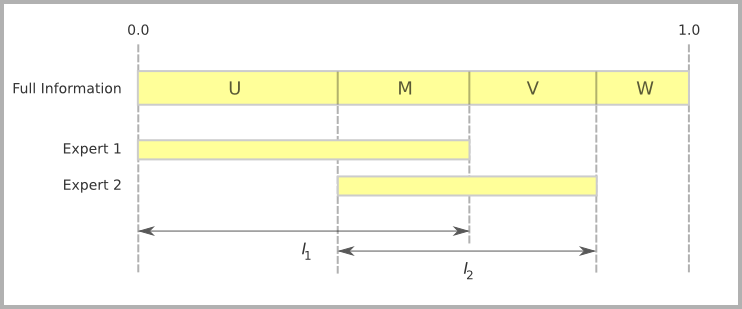
\includegraphics[width = \textwidth]{N=2} % requires the graphicx package
   \caption{Illustration of the partial information model with $2$ forecasters.}
   \label{diagram2}
\end{figure}
Figure \ref{diagram2} illustrates this setup.  In this diagram the 
Gaussian process has been partitioned into four parts based on the 
forecasters' information sets:
\begin{align*}
 U &= X_{I_1 / I_2}
& M &= X_{I_1 \cap I_2}\\
 V &= X_{I_2 / I_1}
& W &= X_{(I_1 \cup I_2)^c}
\end{align*}
Then,
\begin{align*}
X_{I_1} &= U + M\\
X_{I_2} &= M + V\\
X_S &= U+M+V+W,
\end{align*}
where $U, V, M, W$ are independent Gaussians with respective variances 
$\delta_1-\rho$, $\delta_2-\rho$, $\rho$, $1+\rho-\delta_1 - \delta_2$. 
The random variable $X_{I_i}$ can be interpreted as the information 
known by forecaster $E_i$.  The joint distribution of $X_{S}$, $X_{I_1}$, 
and $X_{I_2}$ is a multivariate Gaussian distribution.  That is,
\begin{align}
\left(\begin{matrix} X_S \\ X_{I_1}\\ X_{I_2} \end{matrix}\right) 
 &\sim \mathcal{N}\left(
 \boldsymbol{0},  \left(\begin{matrix} 
1 & \delta_1 & \delta_2\\
\delta_1 & \delta_1 &\rho\\
\delta_2 & \rho & \delta_2
 \end{matrix}\right)\right) \label{twoforecasters}
\end{align}
Given that $X_S$ has mean zero, the prior probability for the event 
is $\P(X_S > 0) = \P(A) = 1/2$.  As mentioned above in (\ref{item:centered}), 
this can be easily adjusted to any probability $\tilde{p}$ by 
letting $A = \{ X_S > \Phi^{-1}(1-\tilde{p}) \}$.  In this paper
we limit our attention to the centered model, with prior probability $1/2$.

\begin{figure}[htbp]
   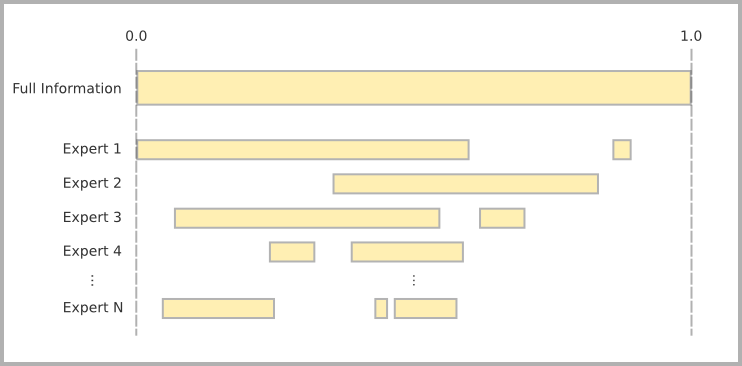
\includegraphics[width = \textwidth]{N=N} % requires the graphicx package
   \caption{Illustration of the partial information model with $N$ forecasters.}
   \label{diagramN}
\end{figure}

Consider now $N$ forecasters. Let $|I_j| = \delta_j$ be the amount of 
information known by forecaster $E_j$ for $j = 1, \dots, N$, and 
$|I_i \cap I_j| = \rho_{ij} = \rho_{ji}$ be the information overlap 
between forecasters $E_i$ and $E_j$ with $i \neq j$. 
Expression~(\ref{twoforecasters}) generalizes to the vector 
$(X_{S}, X_{I_1}, X_{I_2}, \dots, X_{I_N})$ as follows.
\begin{align}
\left(\begin{matrix} X_S \\ X_{I_1}\\ \vdots \\ X_{I_N} \end{matrix}\right) &\sim \mathcal{N}\left( \left(\begin{matrix} 
\mu_1 \\ \boldsymbol{\mu}_2
 \end{matrix}\right) =
 \boldsymbol{0}, \left(\begin{matrix} 
\Sigma_{11} & \Sigma_{12}\\
\Sigma_{21} & \Sigma_{22}\\
 \end{matrix}\right) 
 =
 \left(\begin{array}{c | c c cc }
1 & \delta_1 & \delta_2 & \dots & \delta_N  \\ \hline
\delta_1 & \delta_1 &\rho_{1,2} & \dots & \rho_{1,N}   \\ 
\delta_2 & \rho_{2,1} & \delta_2 & \dots & \rho_{2,N}  \\ 
\vdots & \vdots & \vdots & \ddots & \vdots  \\ 
\delta_N & \rho_{N,1} & \rho_{N,2} & \dots & \delta_N\\ 
 \end{array}\right)\right)  \label{Nforecasters}
\end{align}
This case is illustrated in Figure \ref{diagramN}.  It is important 
to notice that $I_j$ does not have to be a contiguous segment of 
the unit interval.  Instead, each forecaster can know any Borel measurable 
subset of the full information.  Given that the information structure 
is described by the sub-matrix $\Sigma_{22}$, learning about the 
information among the $N$ forecasters is equivalent to estimating 
a covariance matrix under several restrictions.  First, each element 
of $\Sigma_{22}$ must be in the unit interval, and no off-diagonal 
element can be larger than the corresponding diagonal element in 
the same row. Second, $\Sigma_{22}$ must be symmetric, non-singular, 
and coherent. The matrix $\Sigma_{22}$ is coherent if and only if 
its information structure can be described by a diagram such as 
the one given in Figure \ref{diagramN}. 


The next step is to link this model with the probability forecasts. 
If $P_{I_i} = X_{I_i}/\sqrt{1-\delta_i}$ represents $E_i$'s probit 
forecast, the corresponding probability forecast is given by
\begin{align}
p_i &= \P\left(A | \mathcal{F}_{I_i}\right) = \Phi\left( P_{I_i}\right) 
\label{Indiv}
\end{align}
These forecasts are calibrated. 
%Let $A_1, A_2, \dots$ be a infinite sequence of events, each defined 
%similarly to $A$.  If the $i$th forecaster's probability forecast for 
%$A_j$ is given by~(\ref{Indiv}), then the forecaster's forecasts are
%calibrated.  Given that several experiments have shown that forecasters 
%are often poorly calibrated (see, e.g.,~\citealt{cooke1991forecasters, 
%shlyakhter1994quantifying}), assuming calibrated forecasts can be 
%unrealistic.  If the forecasters make repeated forecasts for a sequence 
%of events (e.g., whether it rains or not over a series of days), 
%it may be possible to calibrate their forecasts (see, 
%e.g.,~\citealt{foster1998asymptotic, Brier}).  If calibration is not 
%possible, systematic bias can be introduced in the model by 
%changing the total information by an amount unknown to the forecasters. 
%Another alternative is to include an additive error term 
%in~(\ref{Indiv}) such that the forecasters are on average calibrated. 
%These extensions, however, are beyond the scope of this paper. 
The marginal distribution of $p_j$ is
\begin{align*}
m(p_j | \delta_j) &= \sqrt{\frac{1-\delta_j}{\delta_j}} \exp 
   \left\{ \Phi^{-1}(p_j)^2 \left(1-\frac{1}{2 \delta_j} \right) \right\} 
\end{align*}
This is uniform on $[0,1]$ if the forecaster knows half of the information, 
i.e. $\delta_j = 1/2$.  In general the distribution is unimodal with
a minimum at $p = 1/2$ when $\delta > 1/2$ and a maximum at $p = 1/2$
when $\delta < 1/2$.  As $\delta \to 0$ (no information), $p$ converges
to a point mass at $1/2$ (non=informative prediction) and as $\delta \to 1$,
$p$ converges to a correct prediction, whose distribution has atoms of
weight $1/2$ at zero and one. Figure \ref{marginals} illustrates the marginal distribution when $\delta_j$ is equal to $0.3$, $0.5$, and $0.7$. 

\begin{figure}[t]
\centering
	\hspace{0em}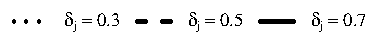
\includegraphics{LegendMarginal}

 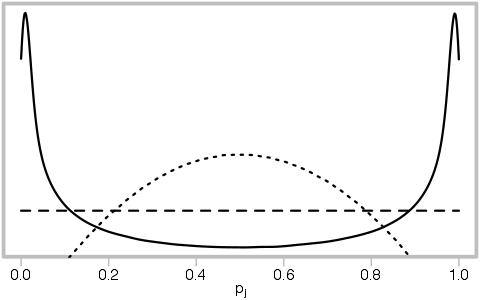
\includegraphics[width= 0.55\textwidth]{Marginals}
   \caption{The marginal distribution of $p_j$ under different levels of 
$\delta_j$.  The more the forecaster knows, i.e. the higher $\delta_j$ is, 
the more the probability forecasts are concentrated around the extreme 
points 0 and~1.}
\label{marginals}
\end{figure}

\section{Probability Extremizing}
\label{extremizing}

This section compares the probit opinion pool aggregator $\probit$ 
to the oracular forecast $p'$. The probit opinion pool was chosen because it is argueably more reasonable than the empirical average, $\bar{p}$. It is very similar to the logarithmic opinion pool but leads to more convenient notation. We show that, under two specific Gaussian partial 
information models, the oracle, on average,
extremizes the probit aggregator.  Recall that the oracle is emulated
by a forecaster whose information set is $I' := \bigcup_{i=1}^N I_i$.
Appending to the multivariate Gaussian distribution~(\ref{Nforecasters}),
\begin{align}
\left(\begin{matrix} X_S \\ X_{I'} \\ X_{I_1}\\ \vdots \\ X_{I_N} 
 \end{matrix}\right) &\sim \mathcal{N}\left( 
 \boldsymbol{0}, \left(\begin{matrix} 
\Sigma_{11}' & \Sigma_{12}'\\
\Sigma_{21}' & \Sigma_{22}\\
 \end{matrix}\right) 
 =
 \left(\begin{array}{c c| c c cc }
1 & \delta' & \delta_1 & \delta_2 & \dots & \delta_N  \\ 
\delta' & \delta' & \delta_1 & \delta_2 & \dots & \delta_N  \\ \hline
\delta_1& \delta_1 & \delta_1 &\rho_{1,2} & \dots & \rho_{1,N}   \\ 
\delta_2 & \delta_2 &\rho_{2,1} & \delta_2 & \dots & \rho_{2,N}  \\ 
\vdots &\vdots & \vdots & \vdots & \ddots & \vdots  \\ 
\delta_N &\delta_N & \rho_{N,1} & \rho_{N,2} & \dots & \delta_N\\ 
 \end{array}\right)\right), \label{oracleN} 
\end{align}
where  $X_{I'}$  is the information known by the oracle and $\delta' = |I'|$ is the amount of this information.  Thus,
 \begin{align*}
p' = \P(X_S > 0 |  \mathcal{F}') 
   &= \Phi\left( \frac{X_{I'}}{\sqrt{1-\delta'}} \right)
\end{align*}

We say that a probability $p$ is extremized by another probability $p'$ 
if and only if $p'$ is closer to~$0$ when $p \leq 0.5$ and closer 
to~$1$ when $p \geq 0.5$.  Define the {\em probit extremization ratio}
to be the real number $\alpha := \Phi^{-1}(p') / \Phi^{-1} (p)$; thus,
$p'$ extremizes $p$ when $\alpha > 1$.  In the case where $p = \probit$,
this gives
\begin{align}
\alpha  = \frac{P_{I'}}{\frac{1}{N}\sum_{j=1}^N P_{I_j}}\label{alpha}
\end{align}
%
This is a random quantity that spans the entire real line, that is, 
it is possible to find a set of probability forecasts and a distribution 
of information for any possible value of $\alpha \in \mathbb{R}$. 
Evidently, extremizing is not guaranteed to always improve the 
probit opinion pool.  
To understand when extremizing is likely to be beneficial, 
it is necessary to derive the probability distribution of $\alpha$. 
First, given that 
\begin{align*}
P_{I'} &\sim \mathcal{N}\left(0, \sigma^2_{1} = 
  \frac{\delta'}{1-\delta'} \right)\\ \frac{1}{N}\sum_{j=1}^N P_{I_j} 
&\sim \mathcal{N}\left(0, \sigma^2_{2} =\frac{1}{N^2} 
  \left\{ \sum_{j=1}^N \frac{\delta_j}{1-\delta_j} 
  + 2 \sum_{i,j: i<j} \frac{\rho_{ij}}{\sqrt{(1-\delta_j)(1-\delta_i)}}
  \right\} \right),
\end{align*}
the amount of extremizing $\alpha$ is a ratio of two correlated 
Gaussian random variables.  The Pearson product-moment correlation 
coefficient for them is
\begin{align*}
\kappa  &= 
  \frac{ \sum_{j=1}^N \frac{\delta_j}{\sqrt{1-\delta_j}}}
  {\sqrt{\delta'  \left( \sum_{j=1}^N \frac{\delta_j}{1-\delta_j} + 2 
  \sum_{i,j: i<j} \frac{\rho_{ij}}{\sqrt{(1-\delta_j)(1-\delta_i)}}\right)}}
  \; .
\end{align*}
It follows that $\alpha$ has a Cauchy distribution as long as 
$\sigma_1 \neq 1$, $\sigma_2 \neq 1$, or $\kappa \pm 1$ 
(see, e.g., \citealt{cedilnik2004distribution} for this 
well known result).  These conditions are very mild under 
the partial information model.  For instance, if no forecaster 
knows as much as the oracle, the conditions are satisfied. 
Consequently, the probability density function of $\alpha$ is
\begin{align*}
f(\alpha | x_0, \gamma) &= \frac{1}{\pi} 
  \frac{\gamma}{(\alpha-x_0)^2+\gamma^2}, 
\end{align*}
where 
\begin{align*}
x_0 = \kappa \frac{\sigma_1}{\sigma_2} \hspace{0.2in} \mbox{ and } 
  \hspace{0.2in} \gamma &= \frac{\sigma_1}{\sigma_2} \sqrt{1-\kappa^2} \, .
\end{align*}
The parameter $x_0$ represents the location (the median and mode) and 
$\gamma$ specifies the scale (half the interquartile range) of the 
Cauchy distribution. This leads to the following proposition. 
The proof of this and other propositions are deferred to Appendix A.

\begin{proposition}
\label{positiveProbThm}
The law of the extremization ratio $\alpha$ is a Cauchy with 
parameters $x_0$ and $\gamma$, where the location parameter 
$x_0$ is at least~1, equality occuring only when $\delta_i = \delta'$ 
for all $i = 1, \dots, N$. Consequently, if $\delta_i \neq \delta'$ 
for some $i = 1, \dots, N$, then the probability that the probit 
opinion pool requires extremizing is $\P(\alpha > 1 | \Sigma_{22}, \delta')$
which is strictly greater than $1/2$. 
\end{proposition}
\noindent
This proposition shows that, on any non-trivial problem, a small
perturbation in the direction of extremizing is more likely to 
improve the probit opinion pool than to degrade it.  This partially 
explains why extremizing aggregators perform well on large sets of 
real-world prediction problems.  It may be unsurprising after the fact,
but the forecasting literature is still full of articles that perform 
probability averaging without extremizing.  The next two 
subsections examine simple models in which more detailed 
computations may be performed.  

\subsection{Fully- and Non-Overlapping Information}
\label{disjoint}
This section examines two scenarios, namely, when the forecasters share no information and when the forecasters share all their information. In the latter case, $I_{i} = I_j$ for all $i \neq j$, the oracular and revealed aggregators, $p'$ and $p''$ coincide and equal to all $p_j$ for $j = 1, \dots, N$. Consequently, $\alpha = 1$ and no extremization is needed. Given that the oracular forecast varies smoothly over the space of  information structures, averaging techniques such as the probit opinion pool can be expected to work well when the forecasters are forming their forecasts based on similar information sets.
% For instance, the forecasters may discuss the forecasting problem before making their separate predictions. 


Next assume that the forecasters' information sets do not overlap, 
i.e., $|I_{i} \cap I_{j}| = 0$ for all $i \neq j$. 
% Such an information 
%structure is likely to arise if a team of forecasters strategically decide 
%to access and study disjoint sources of information.
In this situation the oracular and revealed aggregators $p'$ and $p''$
coincide because $p_i$ determines $X_i$ and $X_{I'}$ is the sum of
all the $X_i$.  The resulting information structure $\Sigma_{22}$ 
is diagonal, and hence coherent if and only if $\sum_{j=1}^N \delta_j \leq 1$ 
with all $\delta_j \in [0,1]$.  Given that under non-overlapping information 
$\delta' = \sum_{j=1}^N \delta_j$ and $X_{I'} = \sum_{j=1}^N X_{I_j}$, 
 \begin{align}
p' &= \Phi\left( \frac{\sum_{j=1}^N X_{I_j}}
  {\sqrt{1- \sum_{j=1}^N \delta_j}} \right) \label{vote}
\end{align}
This aggregator can be described in two steps: The first step consists of voting where votes are weighted according to the importance of the forecasters' private information. This is performed by the summation in the numerator. If this sum falls below $0.0$ (or above $0.0$), the consensus believes that the event will not happen (or will happen). The second step is performed by the denominator that extremizes the forecasters'  consensus belief according to the total amount of information in the group. For instance, if the forecasters know all the information, i.e. $\sum_{j=1}^N \delta_j = 1$, their vote deterministically indicates whether the event $A$ happens or not.  Therefore voting-like techniques can be expected to work well if the forecasters form their forecasts based on largely different information sets. 

%Combining this with our earlier discussion leads to the following observation.
The analysis suggests a spectrum of aggregators indexed by the 
information overlap.  Averaging the probit forecasts yields an 
optimal aggregate under full information overlap.  The optimal 
aggregator, however, undergoes a smooth transformation from 
averaging to summing of the probit forecasts as the information 
overlap decreases towards the point of no overlap, i.e., as the 
information structure becomes diagonal.  
%This is summarized in the following observation.
%%\begin{observation}
%The information structures index a spectrum of aggregators. 
That is,
\begin{center}
\begin{tabular}{ccc}
%\stackrel{\text{ \normalsize full information overlap}}{\stackrel{\text{\normalsize no extremization}}{averaging}} && \Leftrightarrow  && \stackrel{\text{ no information overlap}}{\text{full extremization}}
%high information overlap & \multirow{2}{*}{$\Leftrightarrow$} & low information overlap\\
high information overlap & & low information overlap\\
low extremization & {\Large $\Longleftrightarrow$} & high extremization \\
averaging  & & voting\\
\end{tabular}
\end{center}
%\end{observation}
This observation gives qualitative
guidance in real world settings where the general level of overlap 
can said to be high or low.  For instance, forecasts from a group 
of forecasters working together or in close collaboration can be 
averaged while forecasts from a diverse group of forecasters working 
independently of each other should be aggregated via more extreme 
techniques such as voting (see \citet{parunak2013characterizing} 
for a discussion on aggregation via voting). The next section examines the intermediate scenarios by assuming constant sharing of information among the forecasters. 

%Because $p_i$ and $X_{I_i}$ are related by the one-to-one 
%transformation~(\ref{Indiv}), we may also write this as
% \begin{align}
%p' &= \Phi \left \{ \frac{1}{\sqrt{1 - \sum_{i=1}^N \delta_i}}
%   \; \sum_{i=1}^N \sqrt{1 - \delta_i} \Phi^{-1} (p_i) \right \} \, .
%\end{align}
%In the appendix we prove the following result.  Note that this 
%result is not distributional, it holds samplewise when all the
%forecasts fall on the same side of $1/2$.
%
%\begin{proposition}
%\label{positiveThmVote}
%Under the non-overlapping information structure, the extremization
%parameter $\alpha$ is at least $1$ either if every $X_{I_i} \geq 0$ 
%or if every $X_{I_i} \leq 0$ (equivalently, if every $p_i \geq 1/2$ 
%or every $p_i \leq 1/2$).
%\end{proposition}

\subsection{Extremizing under Compound Symmetric Information}
\label{compound}

Assume that the forecasters' information sets have the 
same size and that the amount of overlap between any two information 
sets is constant, i.e., $|I_{1}| =  \dots = |I_{N}|$ and 
$|I_{i} \cap I_{j}| = |I_{h} \cap I_{k}|$ for all $i \neq j$ 
and $h \neq k$.  In this case the revealed aggregator is not
as good as the oracular aggregator (the former is a conditional
expectation of the latter).  
%Here, we compare $\probit$ to the
%oracular aggregator; in Section~\ref{compound2}
%we compare the revealed aggregator to the probit opinion pool.
The information structure $\Sigma_{22}$ is compound symmetric.  
This structure would hold, for example, if the forecasters 
sample information sources from a common distribution. 
Assuming compound symmetric information in (\ref{oracleN}) results in
\begin{align}
\label{eq:symmetric}
\left(\begin{matrix} X_{S} \\ X_{I'}\\ X_{I_1}\\ \vdots \\ X_{I_N} 
   \end{matrix}\right) 
  &\sim \mathcal{N}\left( \boldsymbol{0}, \left(\begin{matrix} 
\Sigma_{11}' & \Sigma_{12}'\\
\Sigma_{21}' & \Sigma_{22}\\
 \end{matrix}\right) 
 =
 \left(\begin{array}{cc|cccc}
1 & \delta'& \delta & \delta & \dots & \delta  \\ 
\delta' & \delta' & \delta & \delta & \dots & \delta  \\ \hline
\delta & \delta &\delta & \lambda\delta & \dots & \lambda\delta   \\ 
\delta& \delta & \lambda\delta & \delta & \dots & \lambda\delta  \\ 
\vdots &\vdots & \vdots & \vdots & \ddots & \vdots  \\ 
\delta &\delta & \lambda\delta & \lambda\delta & \dots & \delta\\ 
 \end{array}\right)\right)
\end{align}

The amount of information known by each forecaster is denoted 
by $\delta \in [0,1]$.  The value of $\lambda$ is the proportion 
of the information known to one forecaster that is also known to
another single forecaster.  This minor change of parametrization 
was made for the sake of simplifying some of the following expressions. 
To ensure that $\Sigma_{22}$ is coherent, a restriction must 
be placed on $\lambda$. 
First, given that under any combination of $\delta$ and $N$ all forecasters 
may know the exact same information, the value of $\lambda$ is 
bounded from above by $1$. Second, observe that information overlap 
is unavoidable when $\delta > 1/N$.  The minimum sharing occurs when 
all information is either shared or private.  In other words, 
if $\delta > 1/N$ and $I_{i} \cap I_j = I$ with $|I| =  \lambda \delta$ 
for all $i \neq j$, the value of $\lambda$ is minimized when 
$\lambda\delta + N(\delta - \delta\lambda) = 1$.  Therefore the 
lower bound for $\lambda$ is $\max \left\{ \frac{N-\delta^{-1}}{N-1}, 
0\right\}$, and $\Sigma_{22}$ is coherent if and only if
\begin{align}
\delta \in [0,1] &&  \lambda &\in \left[  
   \max \left\{ \frac{N-\delta^{-1}}{N-1}, 0\right\}, 1 \right), 
   \label{rhoDomain}
\end{align}
where the strict upper bound on $\lambda$ ensures that
$\Sigma_{22}$ is not singular.  In the following discussion, 
however, this technical restriction is ignored and the case 
$\lambda = 1$ is analyzed as a limiting case.
Plugging these simplifications in (\ref{alpha}) gives 
\begin{align*}
\alpha &= \frac{X_{I'}}{\frac{1}{N}\sum_{j=1}^N X_{I_j}} 
  \sqrt{\frac{1-\delta}{1-\delta'}} 
\end{align*}
This follows a $\text{Cauchy}(x_0, \gamma)$ distribution with
\begin{align*}
x_0 &= \frac{N}{1+(N-1)\lambda}  \sqrt{\frac{1-\delta}{1-\delta'}}\\[2ex]
  \gamma &=  \sqrt{\frac{N(\delta' + \delta' \lambda (N-1) - \delta N)}
  {\delta (\lambda (N-1) + 1)^2}}\sqrt{\frac{1-\delta}{1-\delta'}}
\end{align*}
The total amount of information among the forecasters $\delta'$ is uniquely determined by $\delta$ and $\rho$ when the group involves only two forecasters. More specifically, $\delta' = \delta(2 - \lambda)$ when $N=2$. Therefore, by assuming only two forecasters, both $x_0$ and $\gamma$ can be analyzed graphically under different information structures. The analysis is almost fully general because compound symmetry under $N = 2$ forecasters is equivalent to only assuming $\delta_1 = \delta_2$. Figure \ref{LevelplotsOracle} considers only $N=2$ forecasters and shows $\log(x_0)$, $\gamma$, and $\P(\alpha > 1 | \Sigma_{22}, \delta')$ under all plausible combinations of $\delta$ and $\rho$. High values have been censored to keep the scale manageable. 


\begin{figure}[t]
\hspace{-1.2em}
    \centering
    \begin{subfigure}[b]{0.33\textwidth}
        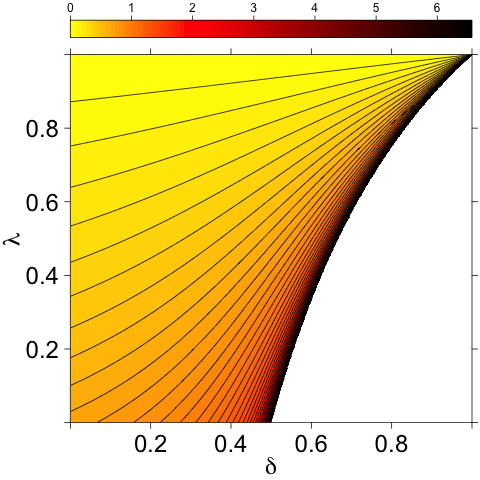
\includegraphics[width=1.07\textwidth, height = \textwidth]{ExtremeX0}
\caption{$\log(x_0)$}	
\label{xOracle}
    \end{subfigure}%
\hspace{0.6em}
    \begin{subfigure}[b]{0.33\textwidth}
        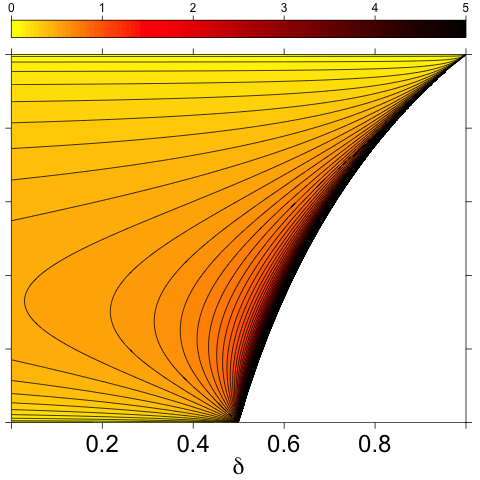
\includegraphics[width= 0.95\textwidth, height = \textwidth]{ExtremeGamma}
\caption{$\gamma$}
\label{gammaOracle}
        \end{subfigure}
\hspace{-1.3em}
    \begin{subfigure}[b]{0.33\textwidth}
        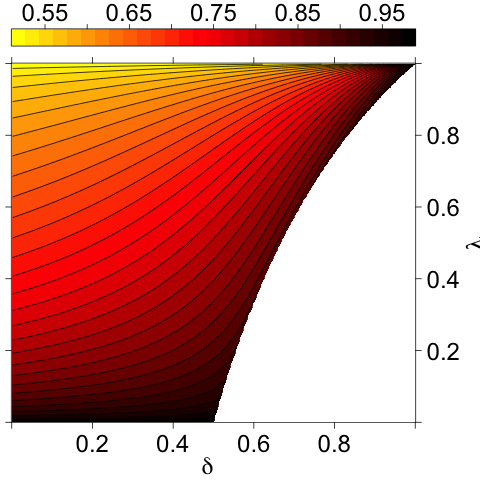
\includegraphics[width=1.07\textwidth, height = \textwidth]{Probs}
\caption{$\P(\alpha > 1 | \Sigma_{22}, \delta')$}
\label{probOracle}
        \end{subfigure}

    \caption{ The amount of extremizing follows a 
Cauchy$(x_0, \gamma)$, where $x_0$ is a location parameter and $\gamma$ 
is a scale parameter.  This figure considers only $N = 2$ forecasters and 
shows $\log(x_0)$, $\gamma$, and $\P(\alpha > 1 | \Sigma_{22}, \delta')$ 
under all plausible combinations of $\delta$ and $\lambda$.}
        \label{LevelplotsOracle}
\end{figure}
 
According to Figure \ref{LevelplotsOracle}, extremizing is required 
more often when $\delta$ is high and $\lambda$ is low.  Given that 
$\delta'$ increases in $\delta$ but decreases in $\lambda$, the amount 
of extremizing can be expected to increase in the total amount of 
information among the forecasters $\delta'$.  This, however, does not 
provide a full explanation of extremizing.  Information diversity 
is also an important yet separate determinant of extremizing.  
To see this, observe that fixing $\delta'$ to some constant 
defines a curve $\lambda = 2 - \delta'/\delta$ on the plots in 
Figure~\ref{LevelplotsOracle}.  For instance, letting $\delta' = 1$ 
gives the boundary curve on the right side of each plot.  This curve 
then shifts inwards and rotates slightly counterclockwise as 
$\delta'$ decreases.  At the top end of each curve all forecasters 
know and share the total information, i.e. $\delta = \delta'$ and 
$\lambda = 1.0$.  At the bottom end, on the other hand, the forecasters 
partition the total information, i.e. $\delta = \delta'/2$, and 
share nothing, i.e. $\lambda = 0.0$.  Given that moving down along 
the curve increases both information diversity and the modal amount 
of extremizing, information diversity is an important determinant 
of extremizing together with the group's total information.  
%This provides the basis for our second observation.
%\begin{observation}
Therefore the amount of extremization can be expected to increases in factors such as number of forecasters, subject-matter forecasterise, and human diversity, but to decrease in collaboration, sharing of resources, and problem difficulty.
%\begin{center}
%\begin{tabular}{l | l}
%increase in & decrease in\\ \hline
%Number of forecasters & Collaboration\\
%Subject-Matter forecasterise & Sharing of Resources\\
%Human Diversity & Problem Difficulty
%\end{tabular}
%\end{center}
%\end{observation}

%Therefore the amount of extremizing can be expected to increase 
%in many factors such as human diversity, subject-matter forecasterise, 
%and the extent to which forecasters can access information, but decrease 
%through forecaster collaboration and sharing of resources. 




\section{Probability Aggregation}
\label{aggregation}

In this section we compute the revealed aggregator $p''$ for 
the general Gaussian partial information model.  We then apply 
this to the symmetric case, for which the oracular aggregator 
was discussed in Section~\ref{compound}.  The revealed aggregator, 
unlike the oracular aggregator, can be applied in practice.  
We prove an extremizing result for this aggregator.

\subsection{Revealed aggregator for the Gaussian model}

Referring back to (\ref{Nforecasters}), if $\boldsymbol{X} = 
(X_{I_1}, X_{I_2},  \dots, X_{I_N})'$ is a column vector 
of length $N$ and $\Sigma_{22}$ is a coherent overlap structure 
such that $\Sigma_{22}^{-1}$ exists, then 
\begin{align*}
X_{S} | \boldsymbol{X} \sim \mathcal{N}\left(\bar{\mu}, \bar{\Sigma}\right), 
\end{align*}
where
\begin{align*}
\bar{\mu} &= \mu_1 + \Sigma_{12} \Sigma_{22}^{-1} 
  (\boldsymbol{X} - \boldsymbol{\mu}_2) 
  = \Sigma_{12} \Sigma_{22}^{-1} \boldsymbol{X} \\
 \bar{\Sigma}&= \Sigma_{11} - \Sigma_{12} \Sigma_{22}^{-1} \Sigma_{21} 
 = 1 - \Sigma_{12} \Sigma_{22}^{-1} \Sigma_{21}   \, .
\end{align*}
These expressions can be found directly from the formulas for
the conditional multivariate Gaussian distribution (see, 
e.g.,~\citealt[Result~5.2.10, page~156]{ravishanker2001first}). 
This then leads to a probability aggregator that depends on 
$\Sigma_{22}$.  More specifically, the revealed aggregator is
\begin{eqnarray}
p'' & = & \P\left(A  | \boldsymbol{X}\right)  \nonumber \\
%%%& = & \P\left(X_{S} > 0 | \boldsymbol{X}\right) \nonumber \\
&=& \Phi\left( \frac{\Sigma_{12} \Sigma_{22}^{-1} \boldsymbol{X}}
   {\sqrt{1 - \Sigma_{12} \Sigma_{22}^{-1} \Sigma_{21}}}\right) 
\label{GeneralAggregator} \, .
\end{eqnarray}
Furthermore, if $\one_N$ is a column vector of ones and 
$\boldsymbol{P} = (P_{I_1}, P_{I_2}, \dots, P_{I_N})'$, 
then the extremization parameter for $p''$ with respect to
$\probit$ is given by 
\begin{align*}
\alpha  &= \frac{N \Sigma_{12} \Sigma_{22}^{-1} 
  \boldsymbol{X}}{\left(\boldsymbol{1}_N' \boldsymbol{P} \right) 
  \sqrt{1 - \Sigma_{12} \Sigma_{22}^{-1} \Sigma_{21}}}  \, .
\end{align*}

To make practical use of this computation, one needs values
for the entries of $\Sigma_{22}$.  As discussed in 
Remark~\ref{item:specific} in Section~\ref{ss:Gaussian},
this may be done in one of three ways: by assumption, 
by estimation or in a Bayesian manner.  If one is to assume
a structure, the most natural and non-informative choice is
the symmetric one, to which we now turn.


\subsection{Aggregation under Compound Symmetric Information}
\label{compound2}

In this section we assume symmetry, meaning that ${\bf X}$ and
$\Sigma$ are given by~\eqref{eq:symmetric}.  This assumption
on the parameters of the model corresponds to a type of exchangeability
assumption on the forecasters.  While this is somewhat idealized,
it is a reasonable choice in a low-information environment, for
example when there is no historical or self-report data to
distinguish the forecasters.  The classical aggregators described in 
Section~\ref{sec:prior}, for instance, are symmetric; therefore,
to the extent that they reflet an underlying model, the model 
assumes exchangeability.

Under this assumption, the general aggregator~(\ref{GeneralAggregator}) 
simplifies to
\begin{align}
\P\left(X_S > 0 | \boldsymbol{X}\right) 
  &=\Phi\left(\frac{\frac{1}{(N-1)\lambda +1} 
  \sum_{j=1}^N X_{I_j} }{\sqrt{1- \frac{N\delta}{(N-1)\lambda +1} }}  
  \right) \, . \label{CompoundAggre}
\end{align}
Recall from section \ref{compound} that $\delta \in [0,1]$ can be 
interpreted as the average amount of information known by an forecaster, 
and $\lambda$ is the average proportion of the known information shared 
between any two forecasters.  The domain restriction (\ref{rhoDomain}) 
ensures that the term under the square-root in (\ref{CompoundAggre}) 
is always non-negative.

Given these interpretations, it may at first seem surprising that 
the values of $\delta$ and $\lambda$ can be estimated in practice. 
Intuitively, the estimation relies on two key aspects of the model: 
a) the further the forecast is from the non-informative prior 
(typically at $0.5$), the more informed the forecaster is likely to be 
(see Figure~\ref{marginals}); and b) the more similar any two forecasts 
are, the more information overlap the corresponding forecasters are likely 
to have. This provides enough leverage to estimate $\delta$ and $\lambda$   
via the maximum likelihood method.  Complete technical details and 
instructions for this are provided in Appendix A.  Besides exchangeability, 
the partial information aggregator (\ref{CompoundAggre}) is based on 
very different modeling assumptions than the classical aggregators 
described in Section~\ref{sec:prior}. This makes it more appropriate 
for combining interpreted forecasts as is stated in the following 
proposition.

\begin{proposition} \label{positiveThm}
$(i)$ The extrimzation parameter in the symmetric case is given by
\begin{eqnarray}
\alpha & = & \frac{\displaystyle{\frac{N\sqrt{1-\delta}}{(N-1)\lambda +1}}}
  {\displaystyle{\sqrt{1- \frac{N\delta}{(N-1)\lambda +1} }}} 
  \label{CompoundAlpha} \\[2ex]
& = & \frac{\gamma \sqrt{1 - \delta}}{\sqrt{1-\delta\gamma}} \nonumber \, ,
\end{eqnarray}
where 
$$\gamma = \frac{N}{(N-1)\lambda +1 \, .}$$
$(ii)$ Under the compound symmetric information structure, 
the partial information aggregator extremizes the probit opinion 
pool as long as $p_j \neq p_i$ for some $j \neq i$. \\[2ex]
$(iii)$ the revealed aggregator can leave the convex hull of the 
individual probability forecasts. 
\end{proposition}

This is a non-random quantity that depends only on three 
parameters.  Therefore it can be conveniently analyzed graphically. 
Figure~\ref{Levelplots} considers $N = 2$ and $N = 10$ forecasters, 
and describes the amount of log-extremizing $\log(\alpha)$ under 
all plausible combinations of $\lambda$ and $\delta$.  High values 
have been censored to keep the scale manageable.  Even though the 
patterns in Figure \ref{Levelplots} are very similar to the ones 
shown earlier in Figure~\ref{LevelplotsOracle}, comparing 
$\alpha$ under $N = 2$ and $N = 10$ leads to new observations. 
First, holding both $\delta$ and $\lambda$ fixed, the amount of 
extremizing $\alpha$ increases in $N$.  This can be considered as 
being caused by an increase in the total amount of information 
among the forecasters because $\delta'$ increases in $N$.  Second, 
in general, having many forecasters, each with a considerable amount 
of information, simply leads to unavoidable information overlap. 
This is illustrated in Figure~\ref{Levelplots} where the set of 
possible values of $\lambda$ decreases very rapidly as $\delta$ 
increases. Furthermore, moving from Figure~\ref{ExtremeN2} to 
Figure \ref{ExtremeN10} illustrates how the dependence between 
$\lambda$ and $\delta$ strengthens as $N$ increases.  In fact, 
based on the domain restriction (\ref{rhoDomain}), the value of 
$\lambda \to 1$ as $N \to \infty$ under any given $\delta$. 
Therefore in the limit the group of forecasters is equivalent to 
a single forecaster.  The compound symmetric information structure, 
however, is almost fully general when $N = 2$.  Therefore assuming 
compound symmetric information can be appropriate for small numbers 
of forecasters but becomes restrictive as more forecasters enter the group. 

\begin{figure}[ht!]
\centering
\hspace*{1.2em} 	
\includegraphics[width=0.973\textwidth, height = 3em]{colorkey} 
    \centering
    \begin{subfigure}[b]{0.499\textwidth}
        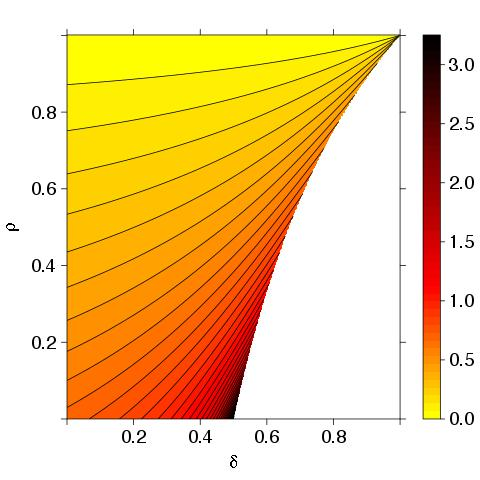
\includegraphics[width=\textwidth]{ExtremeN2}
\caption{N = 2}	
\label{ExtremeN2}
    \end{subfigure}%
    \begin{subfigure}[b]{0.499\textwidth}
        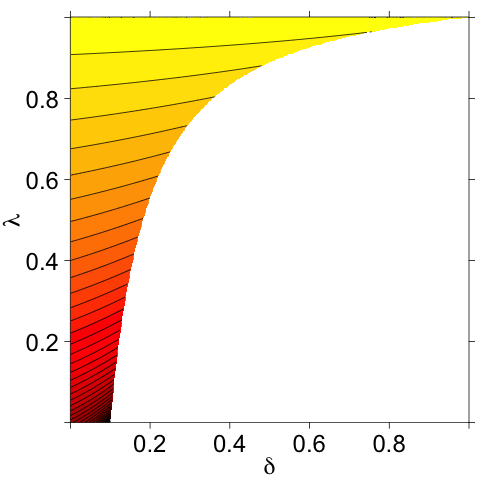
\includegraphics[width=\textwidth]{ExtremeN10}
\caption{N = 10}
\label{ExtremeN10}
    \end{subfigure}
    \caption{ The amount of log-extremizing $\log(\alpha)$ under 
    different combinations of $N$ (the number of forecasters), 
    $\delta$ (the average amount known by one forecaster), and 
    $\lambda$ (the average amount shared by any two forecasters).}
    \label{Levelplots}
\end{figure}
\clearpage

 
\section{Discussion}
\label{discussion}

This paper introduced a probability model for event forecasts made 
by a group of forecasters.  This model allows for interpretation
of some existing work on forecast aggregation.  It also sheds 
light on empirical approaches to forecast aggregation, and in 
particular on the {\em ad hoc} practice of extremization.  

The general model is more plausible on the micro-level than has
been any other model to date.  Under only these general assumption, 
we showed that an oracle would always give a forecast more extreme 
than one of the common benchmark forecasts, namely the probit
opinion pool (Proposition~\ref{positiveProbThm}).  While no 
real world aggregator has access to all the information of the 
oracle, the result nevertheless shows why extremization is almost 
certainly called for.  We gave more detailed analyses under various
specific model specifications, in particular, under the assumptions
of zero information overlap (Section~\ref{disjoint}) and full
symmetry of the information structure (Section~\ref{compound}).
While the zero information overlap model is not realistic, except
under a very narrow set of circumstances, it is a logical extreme
that sheds light on what drives good aggregation and the practice
of extremization (Porposition~\ref{positiveThmVote}.  The symmetric 
model is somewhat more realistic.  Based on its analysis, we 
constructed graphs that illuminated the effect of model parameters 
on the optimal amount of extremization (Figure~\ref{LevelplotsOracle}).
We also considered the {\em revealed aggregator}, which is the
best in-practice aggregation under the partial infomration model.
We derived a general formula for this aggregator 
(Equation~\ref{GeneralAggregator}), as well as its specific formula 
under the assumption of complete symmetry (Equation~\ref{CompoundAggre}).

It is interesting to relate our discussion to the many empirical 
studies conducted by the Good Judgment Project %%%(GJP) 
(\citealt{mellers2014psychological, ungar2012good}).  The GJP is 
a research study that has recruited thousands of forecasters 
from professional societies, research centers, and alumni associations. 
These forecasters are given questions about future international 
political events, such as who would win an election in Russia or 
the Congo.  Individuals then estimate the probability of each event, and 
update their predictions when they feel the probabilities have changed.  
The forecasters know that their probability estimates are assessed 
for accuracy using Brier scores, i.e. the squared distance from the  
probability forecast to $1$ or $0$ depending on whether the event 
happened or not, respectively (\citealt{Brier}).  This incentivizes 
the forecasters to report their true beliefs instead of attempting 
to game the system (\citealt{winkler1968good}).  In addition to receiving 
\$150 for meeting minimum participation requirements that do not depend 
on prediction accuracy, the forecasters receive status rewards for 
their performance via leader-boards displaying Brier scores for the 
top 20 forecasters.  Every year the top 2\% percent of the forecasters 
are selected to the elite group of ``super-forecasters''.  The 
super-forecasters work in groups to make highly accurate predictions 
on the same events as the rest of the forecasters. 

Generally extremizing has been found to improve the average 
aggregates (\citet{mellers2014psychological}).  The average 
forecast of a team of super-forecasters, however, often 
requires very little or no extremizing.  This can explained by 
the partial information model as follows.  The super-forecasters 
are highly knowledgeable (i.e. they have a high $\delta$) 
and they who work in groups (i.e. they have a high $\rho$ and 
$\lambda$).  In Figures~\ref{LevelplotsOracle} and~\ref{Levelplots} 
they are situated around the upper-right corners where almost 
no extremizing is required.  In other words, there is very little
usable information not already used in each forecast.  Ther
forecasts are highly convergent and are already very likely near
the oracular forecast.  The GJP forecast data also includes 
self-assessments of forecasterise.  Not surprisingly, the greater
the self=assessed forecasterise, the less extrimizing appears to 
have been required.  This is consistent with our interpretation
that high values of $\delta$ and $\lambda$ lead to a lower
extremization parameter.

The partial information model offers many future research directions. 
One involves estimation of parameters.  It seems likely that use of
this model together with good procedures for estimating the information
overlap among two or more forecasters could beat current benchmarks
in forecast aggregation.  In the appendix, we discuss means of 
estimating $B_i$ and $|B_i \cap B_j|$ given a stream of forecasts
of reasonable length.  The size of $B_i$ can be estimated from 
the distribution of the forecasts $p_{ij}$ and the size of 
$B_i \cap B_j$ from correslations between the $i$th and $j$th 
forecast streams.  Estimation of higher order intersections seems
more dubious.  Computations with $N=3$ show that, at least in some
cases, higher order intersections are not relevant to the
revealed aggregator.  Theoretical results on the significance or 
insignificance of higher order intersections in the information 
overlap structure would be desirable.

A second promising avenue is the Bayesian approach.  Two forecasters
whose forecasts are very similar or perhaps identical are more
likely to have very similar information sets.  In a Bayesian model,
one would expect more extremization from the probit opinion pool
when the set of forecasts is varied than when it is relatively
homogeneous.  We have work in progress analyzing a Bayesian model
with two forecasters, but there are many, many reasonable priors 
on information structures.  This avenue should certainly be 
pursued and the results tested against other high performing 
aggregators.

\appendix 
\section*{Appendix A: Technical Details}
\label{appendix}

\subsection*{A.1  Proofs}
%\textit{Proof of Theorem \ref{positiveThmVote}.} Let $\boldsymbol{d} = \frac{1}{N}\left((1-\delta_1)^{-1/2}, (1-\delta_2)^{-1/2}, \dots, (1-\delta_N)^{-1/2}\right)'$. Assume without loss of generality that $\bar{P} > 0$. Then the average probit forecast is extremized if
%\begin{align}
% \bar{P}&\leq  \frac{\sum_{j=1}^N X_{I_j}}{\sqrt{1 - \sum_{j=1}^N \delta_j}} &\Leftrightarrow&& 0 \leq  \left\{  \left(1 - \sum_{j=1}^N \delta_j \right)^{-1/2} \boldsymbol{1}_N - \boldsymbol{d}' \right\} \boldsymbol{X} \label{votingproof}
%\end{align}
% As $N (1-\delta_j)^{1/2} \geq \left(1 - \sum_{j=1}^N \delta_j \right)^{1/2}$ for all $j = 1, \dots, N$, all the elements of $$\left(1 - \sum_{j=1}^N \delta_j \right)^{-1/2} \boldsymbol{1}_N - \boldsymbol{d}' $$ are non-negative. Therefore the right hand side of (\ref{votingproof}) is always non-negative. \qed
% \\
% \\
%\noindent

\textit{Proof of Proposition \ref{positiveProbThm}.}
\begin{align*}
x_0 &= \kappa \frac{\sigma_1}{\sigma_2} \\
 &= \frac{ \sum_{j=1}^N \frac{\delta_j}{\sqrt{1-\delta_j}}}{\sqrt{\delta'  \left\{ \sum_{j=1}^N \frac{\delta_j}{1-\delta_j} + 2 \sum_{i,j: i<j} \frac{\rho_{ij}}{\sqrt{(1-\delta_j)(1-\delta_i)}}\right\}}} \sqrt{\frac{\frac{\delta'}{1-\delta'}}{\frac{1}{N^2} \left\{ \sum_{j=1}^N \frac{\delta_j}{1-\delta_j} + 2 \sum_{i,j: i<j} \frac{\rho_{ij}}{\sqrt{(1-\delta_j)(1-\delta_i)}}\right\} }}\\
%&=  \frac{N \sum_{j=1}^N \frac{\delta_j}{\sqrt{1-\delta_j}}}{\sqrt{ \left( \sum_{j=1}^N \frac{\delta_j}{1-\delta_j} + 2 \sum_{i,j: i<j} \frac{\rho_{ij}}{\sqrt{(1-\delta_j)(1-\delta_i)}}\right)}} \sqrt{\frac{\frac{1}{1-\delta'}}{ \left( \sum_{j=1}^N \frac{\delta_j}{1-\delta_j} + 2 \sum_{i,j: i<j} \frac{\rho_{ij}}{\sqrt{(1-\delta_j)(1-\delta_i)}}\right) }}\\
%&=  \frac{N \sum_{j=1}^N \frac{\delta_j}{\sqrt{1-\delta_j}}}{ \sum_{j=1}^N \frac{\delta_j}{1-\delta_j} + 2 \sum_{i,j: i<j} \frac{\rho_{ij}}{\sqrt{(1-\delta_j)(1-\delta_i)}}} \sqrt{\frac{1}{1-\delta'}}\\
&=  \frac{N \sum_{j=1}^N \frac{\delta_j}{\sqrt{(1-\delta_j)(1-\delta')}}}{ \sum_{j=1}^N \frac{\delta_j}{1-\delta_j} + 2 \sum_{i,j: i<j} \frac{\rho_{ij}}{\sqrt{(1-\delta_j)(1-\delta_i)}}}
%&\geq  1
%&=  \frac{\frac{1}{N} \sum_{j=1}^N \frac{\delta_j}{\sqrt{(1-\delta_j)(1-\delta')}}}{\frac{1}{N^2} \left( \sum_{j=1}^N \frac{\delta_j}{1-\delta_j} + 2 \sum_{i,j: i<j} \frac{\rho_{ij}}{\sqrt{(1-\delta_j)(1-\delta_i)}} \right)}\\
\end{align*}
Given that all the remaining terms are positive, the location parameter $x_0$ is also positive. Next compare the $N$ terms with a given subindex $j$ in the numerator with the corresponding terms in the denominator. From $\delta' \geq \delta_j \geq \rho_{ij}$ it follows that 
\begin{align}
\frac{\delta_j}{1-\delta_j} = \frac{\delta_j}{\sqrt{(1-\delta_j)(1-\delta_j)}} &\leq \frac{\delta_j}{\sqrt{(1-\delta_j)(1-\delta')}} \label{ProofIneq1}\\
 \frac{\rho_{ij}}{\sqrt{(1-\delta_j)(1-\delta_i)}} &\leq \frac{\delta_j}{\sqrt{(1-\delta_j)(1-\delta')}} \label{ProofIneq2}
\end{align}
Therefore 
\begin{align*}
N \sum_{j=1}^N \frac{\delta_j}{\sqrt{(1-\delta_j)(1-\delta')}} \geq \sum_{j=1}^N \frac{\delta_j}{1-\delta_j} + 2 \sum_{i,j: i<j} \frac{\rho_{ij}}{\sqrt{(1-\delta_j)(1-\delta_i)}},
\end{align*}
which gives that $x_0 \geq 1$. Given that the Cauchy distribution is symmetric around $x_0$, it must be the case that $\P(\alpha \geq 1 | \Sigma_{22}, \delta') \geq 0.5$. Based on (\ref{ProofIneq1}) and (\ref{ProofIneq2}), the location $x_0 = 1$ only when all the forecasters know the same information, i.e. when $\delta_j = \delta'$ for all $j = 1, \dots, N$. Under this particular setting, the amount of extremizing $\alpha$ is non-random and always equal to $1.0$. Therefore $\P(\alpha \geq 1 | \Sigma_{22}, \delta') = 1.0$.  Any deviation from this particular information structure makes $\alpha$ stochastic, $x_0 > 1$, and hence $\P(\alpha \geq 1 | \Sigma_{22}, \delta') > 0.5$. If the forecaster's information sets partition the full information, the sum of their probits is always on the correct side of $0.0$. At the same time the oracle deterministically outputs the correct outcome. Consequently, $\alpha = +\infty$ and $\P(\alpha \geq 1 | \Sigma_{22}, \delta') = 1$. Thus $\P(\alpha > 1 | \Sigma_{22}, \delta') \in (0.5, 1.0]$ when $\delta_j \neq \delta'$ for some $j = 1, \dots, N$. \qed
\\
\\
%\noindent
%\textit{Proof of Proposition \ref{positiveThmVote}.} Let $\boldsymbol{d} = \frac{1}{N}\left((1-\delta_1)^{-1/2}, (1-\delta_2)^{-1/2}, \dots, (1-\delta_N)^{-1/2}\right)'$. Assume without loss of generality that $\bar{P} > 0$. Then the average probit forecast is extremized if
%\begin{align}
% \bar{P}&\leq  \frac{\sum_{j=1}^N X_{I_j}}{\sqrt{1 - \sum_{j=1}^N \delta_j}} &\Leftrightarrow&& 0 \leq  \left\{  \left(1 - \sum_{j=1}^N \delta_j \right)^{-1/2} \boldsymbol{1}_N - \boldsymbol{d}' \right\} \boldsymbol{X} \label{votingproof}
%\end{align}
% As $N (1-\delta_j)^{1/2} \geq \left(1 - \sum_{j=1}^N \delta_j \right)^{1/2}$ for all $j = 1, \dots, N$, all the elements of $$\left(1 - \sum_{j=1}^N \delta_j \right)^{-1/2} \boldsymbol{1}_N - \boldsymbol{d}' $$ are non-negative. Therefore the right hand side of (\ref{votingproof}) is always non-negative. \qed
%\\
%\\
\noindent
\textit{Proof of Proposition \ref{positiveThm}.} (a) For a given $\delta$, the amount of extremizing $\alpha$ is minimized when $(N-1)\lambda +1$ is maximized. This happens as $\lambda \uparrow 1$. Plugging this into (\ref{CompoundAlpha}) gives
\begin{align*}
\alpha &= \frac{\frac{N\sqrt{1-\delta}}{(N-1)\lambda +1}}{\sqrt{1- \frac{N\delta}{(N-1)\lambda +1} }}  \downarrow \frac{\sqrt{1-\delta}}{\sqrt{1-\delta }} = 1
\end{align*}
(b) Assume without loss of generality that $\bar{P} > 0$. If $\max\{p_1, p_2, \dots, p_N \} < 1$, then  setting $\delta = 1/N$ and $\lambda = 0$ gives an aggregate probability $p'' = 1$ that is outside the convex hull of the individual probabilities.
\qed

\subsection*{A.2 Parameter Estimation under $N=2$ Forecasters}
The information among $N=2$ forecasters is completely characterized by $\delta_1$, $\delta_2$, and $\rho$. The values of these parameters can be estimated via the maximum likelihood method.  To make this more explicit, observe that the Jacobian for the map $\boldsymbol{P} \to \Phi\left(\boldsymbol{P}\right) = (\Phi(P_1), \Phi(P_2))'$ is
\begin{eqnarray*}
J(\boldsymbol{P}) &=& (2\pi)^{-1} \exp \left( - \frac{\boldsymbol{P}' \boldsymbol{P}}{2}   \right) 
\end{eqnarray*}
%
%$\boldsymbol{P} \sim \mathcal{N}_N\left(\boldsymbol{0}, \Sigma_{22} (1-\delta)^{-1}\right)$ and that
Let $\Sigma_{P} =  \Sigma_{22} (1-\delta)^{-1}$. If $h(\boldsymbol{P})$ denotes the multivariate Gaussian density of $\boldsymbol{P} \sim \mathcal{N}_2\left(\boldsymbol{0}, \Sigma_{P}\right)$,
%by the Inverse Function Theorem 
the density for  $\boldsymbol{p} = (p_1, p_2)'$ becomes
\begin{eqnarray*}
 f\left(\boldsymbol{p} | \delta_1, \delta_2, \rho \right) &=& h(\boldsymbol{P}) J(\boldsymbol{P})^{-1} \bigg|_{\boldsymbol{P} = \Phi^{-1}(\boldsymbol{p})}\\
%&=& \frac{(1-\delta)^{N/2}}{\sqrt{ |\Sigma_{22}|}} \exp\left( -\frac{1}{2} \boldsymbol{P}' (1-\delta)\Sigma_{22}^{-1} \boldsymbol{P} + \frac{\boldsymbol{P}' \boldsymbol{P}}{2}   \right)\\
&=& \frac{1}{\sqrt{ \left|\Sigma_{P}\right|}} \exp\left[ -\frac{1}{2} \Phi^{-1}(\boldsymbol{p})' \left\{\Sigma_{P}^{-1} - I_2 \right\} \Phi^{-1}(\boldsymbol{p})  \right]
\end{eqnarray*}
Assume that the forecasters participated in $K$ problems. If the forecasts given for the $k$th problem are denoted with $\boldsymbol{p}_k$, then the maximum likelihood estimates of $\delta$ and $\lambda$ are obtained from
\begin{align*}
\left(\hat{\delta}_1, \hat{\delta}_2, \hat{\rho}\right) =& \argmax_{\delta_1, \delta_2, \rho} \sum_{k=1}^K \log  f\left(\boldsymbol{p}_k| \delta_1, \delta_2, \rho \right),\\
& \text{s.t. } \nonumber \delta_1, \delta_2 \in [0,1] \text{ and } \lambda \in \left[  \max \left\{\delta_1+\delta_2 - 1,  0\right\}, \min \left\{\delta_1, \delta_2 \right\} \right]
\end{align*}
This works well as long as the forecasters participate in the same set of problems. The forecasters, however, were allowed to choose their problems and therefore generally do not participate in the same set of problems. Disregarding any problems with partial participation would lead to a loss of information. Therefore it is necessary to handle the missing values in some manner. The first step is to assume that the forecasts are missing at random. The likelihood for a unpaired forecast, say $p_1$, then becomes 
\begin{eqnarray*}
 f\left(p_1 | \delta_1, \delta_2, \rho \right) &=& \int_0^1 f\left(\boldsymbol{p} | \delta_1, \delta_2, \rho \right) dp_2
% &=& \int_{\mathbb{R}} \frac{(1-\delta)}{\sqrt{ \left|\Sigma_{22}\right|}} \exp\left[ -\frac{1}{2} \boldsymbol{P}' \left\{ (1-\delta) \Sigma_{22}^{-1} - I_2 \right\} \boldsymbol{P}  \right] dP_2\\
% &=&  \frac{1}{\sqrt{ \left|\Sigma_{P}\right|}} \int_{0}^1 \exp\left[ -\frac{1}{2} \Phi^{-1}(\boldsymbol{p})' \left\{  \Sigma_{P}^{-1} - I_2 \right\} \Phi^{-1}(\boldsymbol{p})  \right] dp_2
\end{eqnarray*}
%Assume that $ \Sigma_{P}^{-1} - I_2$ is invertible and let $\Lambda = ( \Sigma_{P}^{-1} - I_2)^{-1}$. Then,
%\begin{eqnarray*}
% f\left(p_1 | \delta_1, \delta_2, \rho \right) &=&  2\pi \sqrt{ \frac{|\Lambda|}{|\Sigma_{P}|}} \int_{\mathbb{R}} \frac{1}{2\pi \sqrt{|\Lambda|}} \exp\left( -\frac{1}{2} \boldsymbol{P}' \Lambda^{-1} \boldsymbol{P}  \right) dP_2\\
% &=&  2\pi  \sqrt{ \frac{|\Lambda|}{|\Sigma_{P}|}} \phi(p_1 | 0, \Lambda_{11}),
%\end{eqnarray*}
%where $\Lambda_{11}$ is the $(1,1)$th element of $\Lambda$ and $\phi(\cdot | \mu, \sigma^2)$ represents the probability density function of a normal distribution with mean $\mu$ and variance $\sigma^2$.
 Let $\mathcal{K}_{12}$ denote the set of problems in which both forecasters participated. Similarly, let $\mathcal{K}_1$ and $\mathcal{K}_2$ denote the sets of problems in which only Forecaster $1$ and $2$ participated, respectively. The final optimization task then becomes
\begin{align*}
\left(\hat{\delta}_1, \hat{\delta}_2, \hat{\rho}\right) =& \argmax_{\delta_1, \delta_2, \rho} \left\{ \sum_{k \in \mathcal{K}_{12}} \log  f\left(\boldsymbol{p}_k| \delta_1, \delta_2, \rho \right) +  \sum_{r = 1}^2 \sum_{k \in \mathcal{K}_{r}} \log  f\left(p_r| \delta_r, \rho \right)  \right\},\\
& \text{s.t. } \nonumber \delta_1, \delta_2 \in [0,1] \text{ and } \lambda \in \left[  \max \left\{\delta_1+\delta_2 - 1,  0\right\}, \min \left\{\delta_1, \delta_2 \right\} \right]
\end{align*}
%Given that this optimization problem cannot be solved analytically, numerical methods must be used. The feasible set of parameter values is a convex set defined by the intersection of four half-spaces. Therefore the constraints are equivalent to a set of linear inequalities
%\begin{align*}
%-\rho &\leq 0\\
%\delta_1+\delta_2-\rho-1 &\leq 0\\
%\rho - \delta_1 &\leq 0\\
%\rho - \delta_2 &\leq 0
%\end{align*}
%and an adaptive barrier method can be used to solve the maximization problem. 
\subsection*{A.3 Estimation of $\delta$ and $\lambda$}


The values of $\delta$ and $\lambda$ can be estimated via the maximum likelihood method. To make this more explicit, observe that the Jacobian for the map $\boldsymbol{P} \to \Phi\left(\boldsymbol{P}\right) = (\Phi(P_1), \Phi(P_2), \dots, \Phi(P_N))'$ is
\begin{eqnarray*}
J(\boldsymbol{P}) &=& (2\pi)^{-N/2} \exp \left( - \frac{\boldsymbol{P}' \boldsymbol{P}}{2}   \right) 
\end{eqnarray*}
%
%$\boldsymbol{P} \sim \mathcal{N}_N\left(\boldsymbol{0}, \Sigma_{22} (1-\delta)^{-1}\right)$ and that
Let $J_{N \times N}$ represent a $N\times N$ matrix of ones. If $h(\boldsymbol{P})$ denotes the multivariate Gaussian density of $\boldsymbol{P} \sim \mathcal{N}_N\left(\boldsymbol{0}, \Sigma_{22} (1-\delta)^{-1}\right)$,
%by the Inverse Function Theorem 
the density for  $\boldsymbol{p} = (p_1, p_2, \dots, p_N)'$ becomes
\begin{eqnarray*}
 f\left(\boldsymbol{p} | \delta, \lambda \right) &=& h(\boldsymbol{P}) J(\boldsymbol{P})^{-1} \bigg|_{\boldsymbol{P} = \Phi^{-1}(\boldsymbol{p})}\\
%&=& \frac{(1-\delta)^{N/2}}{\sqrt{ |\Sigma_{22}|}} \exp\left( -\frac{1}{2} \boldsymbol{P}' (1-\delta)\Sigma_{22}^{-1} \boldsymbol{P} + \frac{\boldsymbol{P}' \boldsymbol{P}}{2}   \right)\\
&=& \frac{(1-\delta)^{N/2}}{\sqrt{ \left|\Sigma_{22}\right|}} \exp\left[ -\frac{1}{2} \Phi^{-1}(\boldsymbol{p})' \left\{ (1-\delta) \Sigma_{22}^{-1} - I_N \right\} \Phi^{-1}(\boldsymbol{p})  \right],
\end{eqnarray*}
%where $\Phi^{-1}(\boldsymbol{p}) =  (\Phi^{-1}(p_1), \Phi^{-1}(p_2), \dots, \Phi^{-1}(p_N))$. 
%Given that $\Sigma_{22}$ can be written in the form  $\Sigma_{22} = I_N (\delta-\lambda\delta) + J_{N \times N} \lambda\delta$
where
%The determinant and inverse of $\Sigma_{22}$ are
\begin{align}
\left| \Sigma_{22}\right| &= (\delta(1- \lambda))^N \left(1+\frac{N \lambda}{1 - \lambda} \right) \nonumber\\
\Sigma_{22}^{-1} &= I_N \left(\frac{1}{\delta-\lambda\delta} \right) - J_{N \times N} \frac{\lambda}{(1-\lambda)\delta\{1+(N-1) \lambda\}} \label{inverse}
\end{align}
See \citet{rao2009linear} and the supplementary material of \citet{dobbin2005sample} for the derivations of the determinant and inverse of $\Sigma_{22}$, respectively. The maximum likelihood estimates of $\delta$ and $\lambda$ are then obtained from
\begin{align*}
\left(\hat{\delta}, \hat{\lambda}\right) =& \argmax_{\lambda, \delta} \log  f\left(\boldsymbol{p}| \delta, \lambda \right),\\
& \text{s.t. } \nonumber \delta \in [0,1] \text{ and } \lambda \in \left[  \max \left\{ \frac{N-\delta^{-1}}{N-1}, 0\right\}, 1 \right)
\end{align*}
%\textcolor{red}{check if this is a convex program}
Given that this cannot be solved analytically, numerical methods such as a simple grid-search must be used to find $\hat{\delta}$ and $\hat{\lambda}$. 

% 

%\bibliographystyle{Chicago}
%\bibliographystyle{plainnat}
\bibliographystyle{chicago}
\bibliography{biblio}		% expects file ''myrefs.bib''



\end{document}
